\documentclass[12pt,letterpaper]{article}

\usepackage[spanish, es-tabla, es-nodecimaldot]{babel}
\usepackage[utf8x]{inputenc}
\usepackage{amsmath}

\usepackage{hyperref}
%\usepackage{url}
\usepackage{textcomp}
\usepackage{gensymb}
\usepackage[dvipsnames]{xcolor}

\usepackage{parskip}
\usepackage{fancyhdr}
\usepackage{multicol}
\usepackage{vmargin}
\usepackage{setspace}
\usepackage{geometry}

\usepackage{float}
\usepackage{array}
\usepackage{graphicx}
\graphicspath{{Images/}}
\usepackage{wrapfig}
\usepackage{caption}
\usepackage{subcaption}
\usepackage[square, numbers, sort]{natbib}

\usepackage{listings}
\usepackage{color}
%\usepackage[usenames,dvipsnames]{color}
	\definecolor{ocre}{RGB}{42,105,21}
	\definecolor{ocre2}{RGB}{0,102,0}%47,109,130}
	\definecolor{gray2}{gray}{0.95}
	\lstset{
		language={[03]fortran},
		backgroundcolor=\color{gray2},
		basicstyle=\color{black}\small\ttfamily, 
		breakatwhitespace=false,         
		breaklines=true,                 
		captionpos=b,                    
		columns=flexible,
		commentstyle=\color{ocre2}\ttfamily, 
		deletekeywords={...},            
		escapeinside={\%*}{*)},          
		extendedchars=true,             
		frame=single,	                 
		keepspaces=true,                 
		keywordstyle=\color{blue}\bfseries,       
		otherkeywords={*,...},          
		numbers=left,                    
		numbersep=5pt,                   
		numberstyle=\small, 
		rulecolor=\color{black},         
		showspaces=false,                
		showstringspaces=false,          
		showtabs=false,                  
		stepnumber=1,                    
		stringstyle=\normalfont\color{ocre},     
		tabsize=2,	                     
		title=\lstname                  
		}
\definecolor{labelcolor}{RGB}{100,0,0}



\setmarginsrb{2.0cm}{1.0cm}{2.0cm}{2.5cm}{0.5cm}{1cm}{1 cm}{1 cm} %{izq}{up}{der}{down}{Encabezado}

\pagestyle{fancy}
\fancyhf{}
\rhead{Lic. Física}
\lhead{Desarrollo Experimental II}
\cfoot{\thepage}


\title{ Comentarios, Desarrollos u Observaciones  }

\newcommand{\pd}[3] {\left(\frac{\partial #1}{\partial #2}\right)_{#3}}
\newcommand{\pdd}[3] {\left(\frac{\partial^2 #1}{\partial {#2}^2}\right)_{#3}}


\begin{document}


\begin{titlepage}
	\centering
    \vspace*{2cm}
	{\Large Proyecto Final \par}
	\vfill
	{\Large Desarrollo Experimental II \par}
	\vfill
	{\large\ Docente:\\ Dra. Laura Lorenia Yeomans Reyna \par}
    \vfill
    {\large\ \textbf{Simulación de Monte Carlo:}\\ 
    \emph{Exploración de la Ecuación de Van Der Waals}\par}
    \vfill
    {\large\ Alumno:\\ Martín Alejandro Paredes Sosa \par}
	\vfill
	% Bottom of the page
	{\large Semestre: 2018-1\par}
\end{titlepage}

\section{Introducción}
	
	La estructura de un líquido está fuertemente determinada por las interacciones repulsivas de corto alcance, y  los estudios con simulaciones computacionales se han utilizado para mostrar que estas interacciones repulsivas de corto alcance pueden modelarse como de núcleo duro. Para modelar un líquido, sin embargo, se requiere una componente atractiva como parte del potencial de interacción entre las partículas del sistema.  

Una de las ecuaciones de estado más importantes y que históricamente se han plateado para describir a los líquidos y la coexistencia líquido-vapor ha sido la ecuación de estado de Van der Waals \cite{Modern}:

\begin{equation}
	\left( p + \frac{N^2}{V^2}a \right) \left( V -Nb \right) = Nk_B T
	\label{VanDerWaals}
\end{equation}

Esta se puede derivarsre como una aplicación de la teoría de perturbaciones de Zwanzig\cite{Stats}, que permite obtener las expresiones para los coeficientes $a$ y $b$ que coinciden con la propuesta de Van Der Waals \cite{Stats} 

\begin{align}
	a &= -2\pi \int_{\sigma}^{\infty} u^{(1)}(r)r^2dr \label{Coef_A_1} \\
	b &= \frac{2\pi\sigma^3}{3} \label{Coef_B_1}
\end{align}
donde $\sigma$ es el diámetro de la esfera dura y $u^{(1)}(r)$ el potencial de interacción atractivo que se considera como la parte perturbativa del potencial de interacción entre las partículas del sistema. 

\begin{equation}
u(r) = u^{(hs)}(r) + u^{(1)}(r)
\label{PotInter_Base}
\end{equation}
\pagebreak

\section{Contexto}
Para la obtención de \eqref{Coef_A_1}, se asume que:
\begin{equation}
	 g_{hs}\approx
		\left\{
		\begin{aligned}
        	0 & \qquad r\leq \sigma\\
	        1 & \qquad r > \sigma ,
       \end{aligned}
       \right.
       \label{gdrhs}
\end{equation}

Esta aproximación es para muy bajas concentraciones, donde la función de distribución radial de contacto $g_{hs}(\sigma^+) \approx 1$, que corresponde al modelo de Van Der Waals.

En el contexto del ensemble canónico en la Física Estadística, la ecuación de estado se obtiene a partir de:
\begin{equation}
	p = \frac{1}{\beta} \left( \frac{\partial Z_N}{\partial V} \right)_{T}
	\label{EnsembleP}
\end{equation}
Como $g_{hs}(r)$ depende de la concentración, la ecuación de estado es de la forma:

\begin{equation}
	p = p_{hs} - \rho^2\left[ a(\rho) + rho \left( \frac{\partial a(\rho)}{\partial\rho} \right)_T \right] 
	\label{Press}
\end{equation}
\begin{equation}
	p_{hs} = \rho k_B T\left[ 1 +\frac{2}{3}\pi\sigma^3\rho g_{hs}(\sigma^+) \right]
	\label{PressHS}
\end{equation}

\pagebreak


\section{Metodología}
\begin{enumerate}
\item[I.]\textbf{Potencial Perturbativo:} La teoría de Zwangzig no impone ninguna restricción sobre el potencial perturbativo $u^{(1)}(r)$ con tal de que sea atractivo. Entonces, consideremos  como potencial  perturbativo la parte atractiva del modelo de pozo cuadrado:
\begin{equation}
	u^{(1)}(r) =
	\left\{
	\begin{aligned}
        -\varepsilon &  \qquad \sigma < r < \lambda\sigma\\
		0 & \qquad r \geq \lambda\sigma 
    \end{aligned}
    \right.
	\label{Pozo}
\end{equation}

De modo que el potencial de interacción según la ecuación \eqref{PotInter_Base} queda:

\begin{equation}
	u(r)=
	\left\{
	\begin{aligned}
		\infty & \qquad r \leq \sigma \\
        -\varepsilon &  \qquad \sigma < r < \lambda\sigma\\
		0 & \qquad r \geq \lambda\sigma \\
	\end{aligned}
    \right.
	\label{PotInteracTotal}
\end{equation}

\item[II.] \textbf{Reducción de variables} Antes de empezar ha realizar cálculos, se redujeron las ecuaciones, tomando como longitud característica el diámetro $\sigma$ y como energía característica la energía térmica $\beta^{-1}$

Por lo tanto obtenemos las siguientes definiciones:
\begin{align}
	r^* &\equiv \frac{r}{\sigma} \label{rRed} \\
	u^*(r) &\equiv \frac{u(r)}{k_B T} = \beta u(r) \label{potRed}\\
	p^* &\equiv \frac{p\sigma^3}{k_B T} =\beta p\sigma^3 \label{presRed}\\
	T^* &\equiv \frac{k_B T}{\varepsilon} =\frac{1}{\beta \varepsilon} = \frac{1}{\varepsilon^*} \label{TempRed} \\
	n^* &\equiv \sigma^3\rho \label{ConsRed}
\end{align}
 De tal forma que:
\begin{equation}
	u^*(r)=
	\left\{
	\begin{aligned}
		\infty & \qquad r^* \leq 1 \\
        \frac{-1}{T^*} &  \qquad 1 < r^* < \lambda\\
		0 & \qquad r^* \geq \lambda \\
	\end{aligned}
    \right.
	\label{PotInteracTotal_Red}
\end{equation}


Utilizando \eqref{rRed}-\eqref{ConsRed} en \eqref{PressHS} obtenemos:
\begin{align}
\frac{p^*_{hs}}{\beta\sigma^3} &= \frac{n^*}{\beta\sigma^3}\left[ 1 +\frac{2}{3}\pi\sigma^3\frac{n^*}{\sigma^3} g_{hs}(1^+) \right] \nonumber \\
p^*_{hs} &= n^* \left[ 1 +\frac{2}{3}\pi n^* g_{hs}(1^+) \right] \nonumber \\
p^*_{hs} &= n^* \left[ 1 + n^*b^*\right] \label{PressHS_Red}
\intertext{Donde:}
b^* &= \frac{2}{3}\pi g_{hs}(1^+) \label{bstar}
\end{align}
Ahora en \eqref{Press} obtenemos:

\begin{align}
\frac{p^*}{\beta\sigma^3} &= \frac{p^*_{hs}}{\beta\sigma^3} - \left(\frac{n^*}{\sigma^3}\right)^2 \left[ a(n^*) + \frac{n^*}{\sigma^3} \left( \frac{\partial a(n^*)}{\partial\frac{n^*}{\sigma^3}} \right)_{T^*} \right] \nonumber \\
p^* &= p^*_{hs}  - \frac{\beta {n^*}^2}{\sigma^3}\left[ a(n^*) + n^* \left( \frac{\partial a(n^*)}{\partial n^*} \right)_{T^*} \right] \nonumber \\
p^* &= p^*_{hs} - {n^*}^2\left[ \frac{\beta}{\sigma^3}a(n^*) + n^* \left(\frac{\partial\frac{\beta}{\sigma^3}a(n^*)}{\partial n^*}\right)_{T^*}\right] \nonumber \\
p^* &= p^*_{hs} - \left[ a^* + n^* \left(\frac{\partial a^*}{\partial n^*}\right)_{T^*} \right] {n^*}^2 \label{Press_Red}
\intertext{Donde:}
a^* &= \frac{\beta}{\sigma^3}a(n^*) \label{a_star}
\end{align}

\item[III.] \textbf{Parámetro Críticos} 
La Ecuación de Van Der Waals \eqref{VanDerWaals} tiene una temperatura crítica $T_c$.
Cuando $T>T_c$ la ecuación de estado es monovaluada y no hay transiciones al estado liquido. Cuando $T<T_c$, como la ecuación es cubica en $V$, tiene dos extremales que se juntan en $T=T_c$.

Pensando en la ecuación de Van Der Waals como una función del volumen a una temperatura dada $P = P(V;T)$, se tienen dos punto críticos donde se cumple   $\left( \partial_V P \right)_T = 0 $. Conforme $T\rightarrow T_c$ se obtiene un punto de inflexión con coordenadas $(P_c, V_c, T_c)$ donde $\left( \partial^2_V P \right)_T=0$

Partiendo de la ecuación \eqref{VanDerWaals}:
\begin{align}
	P &= \frac{Nk_B T}{V-Nb} - \frac{N^2}{V^2}a	\label{PresVanDerWaals} \\
	\pd{P}{V}{T} &= -\frac{Nk_BT}{(V-Nb)^2} + \frac{2N^2a}{V^3} \label{P_Vdw_Dif} \\
	\pdd{P}{V}{T} &= \frac{2Nk_BT}{(V-Nb)^3} - \frac{6N^2a}{V^4} \label{P_Vdw_Dif2}
\end{align}
Aplicando la condición de punto crítico obtenemos el siguiente sistema de ecuaciones para los coeficientes $a$ y $b$

\begin{align*}
	 -\frac{Nk_BT_c}{(V_c-Nb)^2} + \frac{2N^2a}{V_c^3} &= 0\\
	\frac{2Nk_BT_c}{(V_c-Nb)^3} - \frac{6N^2a}{V_c^4}  &= 0
\end{align*}
Despejamos $a$ de la primera ecuación
\begin{align}
\frac{2N^2a}{V_c^3} &=\frac{Nk_BT_c}{(V_c-Nb)^2} \nonumber \\
a &= \frac{Nk_B T_c}{(V_c-Nb)^2} \frac{V_c^3}{2N^2} \label{adespejada}
\end{align}
Ahora en la segunda ecuación hacemos lo mismo

\begin{align*}
\frac{2Nk_BT_c}{(V_c-Nb)^3} &= \frac{6N^2a}{V_c^4}  \\
a &= \frac{2NK_bT_c}{(V_c-Nb)^3} \frac{V_c^4}{6N^2}
\end{align*}
Igualando obtenemos
\begin{align}
\frac{Nk_B T_c}{(V_c-Nb)^2} \frac{V_c^3}{2N^2} &= \frac{2NK_bT_c}{(V_c-Nb)^3} \frac{V_c^4}{6N^2} \nonumber \\
\frac{V_c^3}{2} &= \frac{2}{V_c-Nb} \frac{V_c^4}{6}  \nonumber \\
V_c-Nb &= \frac{V_c}{6} \nonumber\\
b &= \frac{V_c}{3N} \label{b1}
\end{align}
Sustituimos esto en \eqref{adespejada}
\begin{align}
 a &= \frac{Nk_B T_c}{(V_c- N \frac{V_c}{3N})^2} \frac{V_c^3}{2N^2}  \nonumber \\
 a &= \frac{k_B T_c}{(\frac{2V_c}{3})^2} \frac{V_c^3}{2N} \nonumber \\
 a &= \frac{9k_B T_c}{4V_c^2} \frac{V_c^3}{2N^2} \nonumber \\
 a &= \frac{9}{8}k_B T_c \frac{V_c}{N} \label{a1}
\end{align}
A partir de las ecuaciones \eqref{b1} y \eqref{a1} obtenemos que 
\begin{align}
V_c &= 3Nb \label{Vc} \\
T_c &= \frac{8a}{27k_Bb} \label{Tc}\\
P_c &= \frac{a}{27b^2} \label{Pc}
\end{align}
 Ahora obtendremos las expresiones para las variables termodinámicas criticas de Van Der Waals para el caso de estudio con un potencial perturbativo de pozo cuadrado \eqref{Pozo}. Para esto se utilizamos la ecuación \eqref{Coef_A_1} (pero a la Zwanzig) y el potencial reducido.
\begin{align}
 a^* &= -2\pi \int_1^\infty {u^*}^{(1)}(r^*) g_{hs}(r^*) {r^*}^2 dr^* \nonumber \\
  &=-2\pi  \left[ \int_1^\lambda {u^*}^{(1)}(r^*) g_{hs}(r^*) {r^*}^2 dr^* +\int_\lambda^\infty {u^*}^{(1)}(r^*) g_{hs}(r^*) {r^*}^2 dr^*  \right] \nonumber\\
  &= -2\pi \int_1^\lambda \frac{-1}{T^*} g_{hs}(r^*){r^*}^2d{r^*} \nonumber \\
 a^* &= \frac{2\pi}{T^*} \int_1^\lambda g_{hs}(r^*){r^*}^2d{r^*} \label{a_star_Integral}
\end{align}  

Para el caso Van Der Waals la integral queda:
\begin{equation}
a^* = \frac{2\pi}{3} \frac{\lambda^3-1}{T^*}
\end{equation}
Para el coeficiente $b^*$ se tiene la ecuación \eqref{bstar}. Utilizando la suposición de Van Der Waals, entonces obtenemos \eqref{Coef_B_1}, que en es forma reducida resulta:
\begin{equation}
b^* = \frac{2\pi}{3}
\end{equation}

Por lo tanto, de \eqref{Vc},\eqref{Tc} y \eqref{Pc} se obtiene

\begin{align}
V_c^* &= 2\pi N \label{Vcs} \\
T_c^* &= \frac{8}{27}(\lambda^3 -1) \label{Tcs}\\
P_c^* &= \frac{\lambda^3-1}{18\pi T^*} \label{Pcs}
\end{align}
\begin{itemize}
\item \textbf{Ejemplo:} Veamos de qué orden son los valores para las variables criticas para un sistema dado. Sea $\lambda=1.25$, resulta:
\end{itemize}
\begin{align*}
V_c^* &= 2\pi N  \\
T_c^* &= 0.2824 \\
P_c^* &= \frac{0.0169}{ T^*} 
\end{align*}


\item[IV.]\textbf{Función de Distribución Radial de HS} Ahora utilizamos nuestro código de Monte Carlo, con el cual se realizaron corridas para diferentes concentraciones. A continuación se muestra un gráfico de $g(r)-n^*$ para el modelo de potencial HS solamente.
\begin{figure}[H]
	\centering
	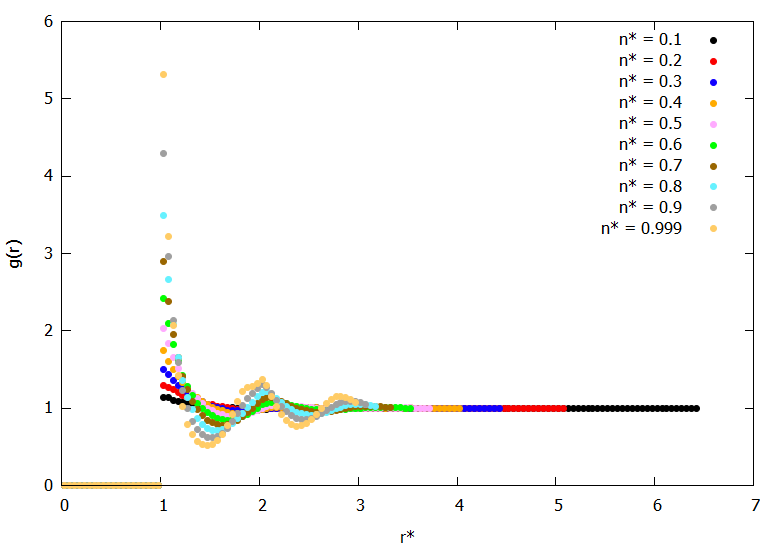
\includegraphics[width=0.75\linewidth]{GDR.png}
	\caption{Función g(r) para potencial de Esfera Dura}
	\label{Fig:GDR_HS}
\end{figure}
 Se pueden apreciar que en el punto de contacto ($r^*4=1$) hay una mayor cantidad de partículas, y esta aumenta junto con la concentración. Los picos muestran la presencia de ``vecinos'' segundos, terceros, etc.
 
 Estos datos se obtuvieron de la Simulación Monte Carlo para un sistema de 216 partículas, se realizaron $3\times10^5$ configuraciones y se considero la configuración $1\times10^5$ como la de equilibrio, para poder olvidar la configuración inicial.

\item[V]\textbf{Ecuación de Presión HS}

En la termodinámica, suele usar la ecuación de de estado de presión contra volumen. Dicho esto, nuestro análisis es $P^*-n^*$ dado la relación que hay entre la concentración y el volumen. Para el estudio de Esferas duras, ya conocemos la ecuación \eqref{PressHS_Red}, junto con \eqref{bstar}. Como $n^*$ es un parámetro conocido de la simulación, basta con conocer el el valor del punto de contacto $g_{hs}(1^+)$

La ecuación de estado de Carnahan-Starling para un sistema de esferas duras está dada por:
\begin{equation}
P^*(n^*) = n^* \frac{1+\phi+\phi^2-\phi^3}{(1-\phi)^3}, \qquad \phi=\frac{\pi}{6} n^*
\end{equation}
En la figura \ref{Fig:EcEstado}, se muestra una comparación entre los datos simulados y las ecuaciones de estado de Gas Ideal y la de Carnahan-Starling.
\begin{figure}[H]
	\centering
	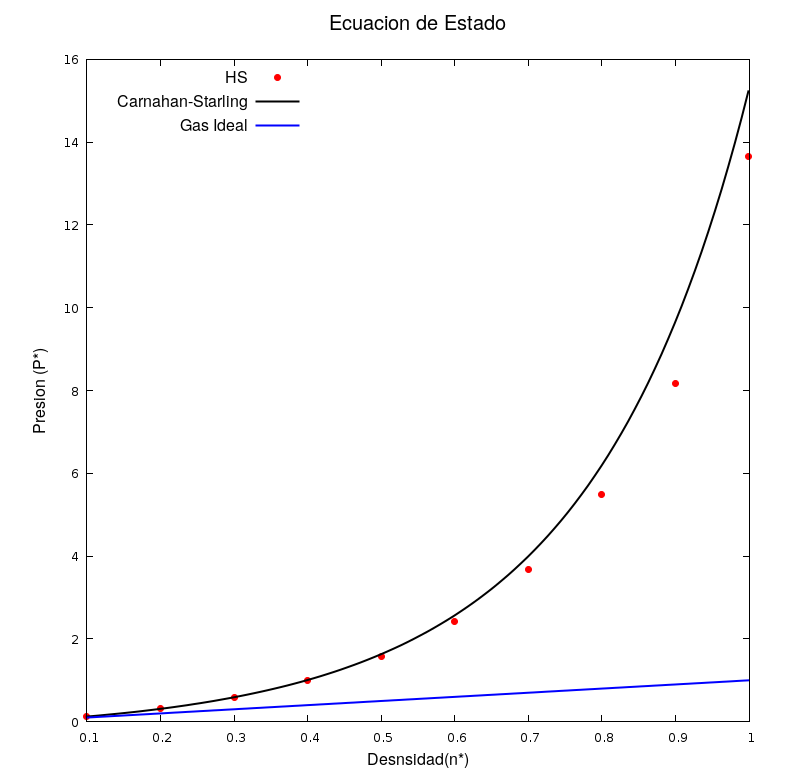
\includegraphics[width=0.75\linewidth]{Comparativo.png}
\caption{Ecuación de Estado de un sistema de esferas duras comparando con la de Gas Ideal y Carnahan Starling}
\label{Fig:EcEstado}
\end{figure}

\item[VI.]\textbf{Calculo de los coeficiente $a^*(n^*)$ y $b^*(n^*)$:}
Con la información estructural que calculamos de las simulaciones (las $g(r^*)$) y p de las ecuaciones \eqref{bstar} y \eqref{a_star_Integral}, se procedió a calcular los coeficientes.
\begin{figure}[H]
	\centering
	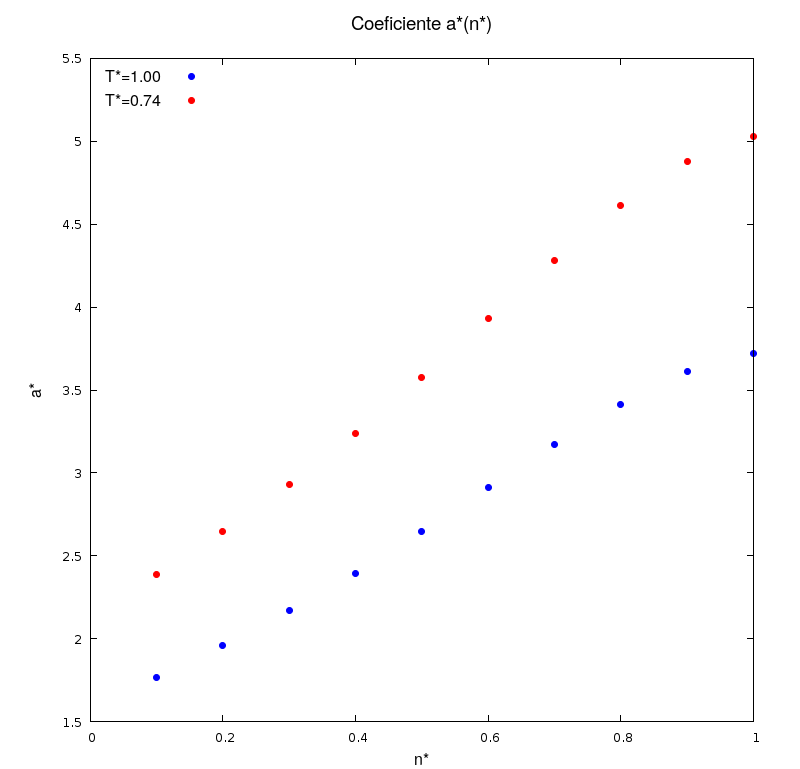
\includegraphics[width=0.65\linewidth]{a_star.png}
	\caption{Coeficiente $a^*$ a $T=1.0$ y $T=0.74$}
	\label{Fig:A_Star}
	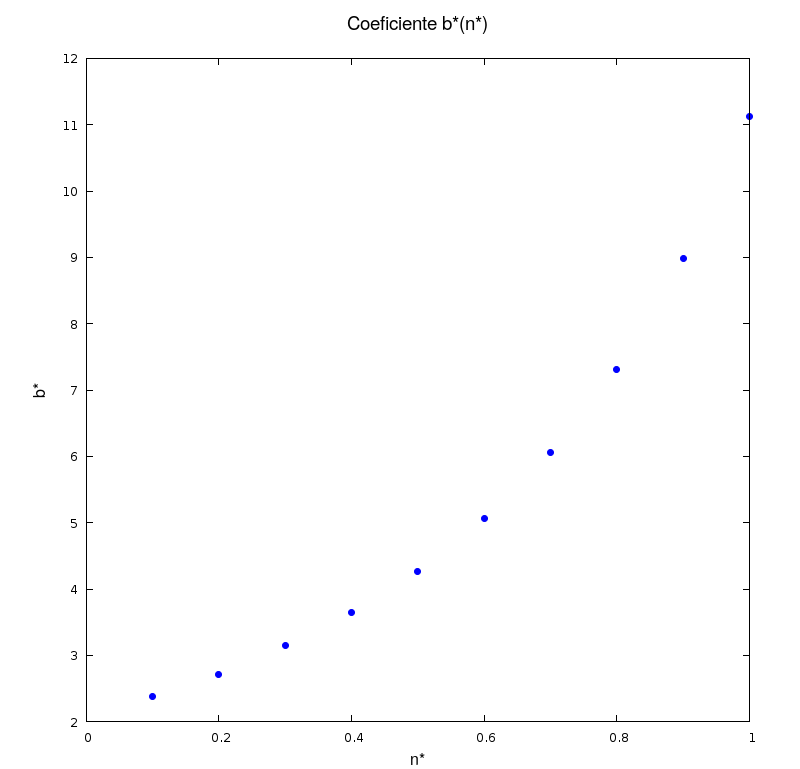
\includegraphics[width=0.65\linewidth]{b_star.png}
		\caption{Coeficiente $b^*$}
	\label{Fig:B_Star}
\end{figure}
 \item[VII.] \textbf{Ajuste de $a^*$ }
De los resultados que obtuvimos de $a^*$, podemos observar una ligera curvatura. Mediante el uso del programa Origin, procedimos a ajustar una curva, que en este caso resulto un polinomio de segundo orden.
Para el caso de $T^*=1.0$ se ajusto lo siguiente:
\begin{align*}
	a^*(n^*) &= 1.47 + 2.48n^* - 0.16 {n^*}^2\\
	\partial_{n^*}a^* &= 2.48 - 0.32n^*
\end{align*}
Y para el caso de $T^*=0.74$
\begin{align*}
	a^*(n^*) &= 1.99 + 3.35n^* - 0.21 {n^*}^2\\
	\partial_{n^*}a^* &= 3.35- 0.42n^*
\end{align*}
\begin{figure}[H]
	\centering
	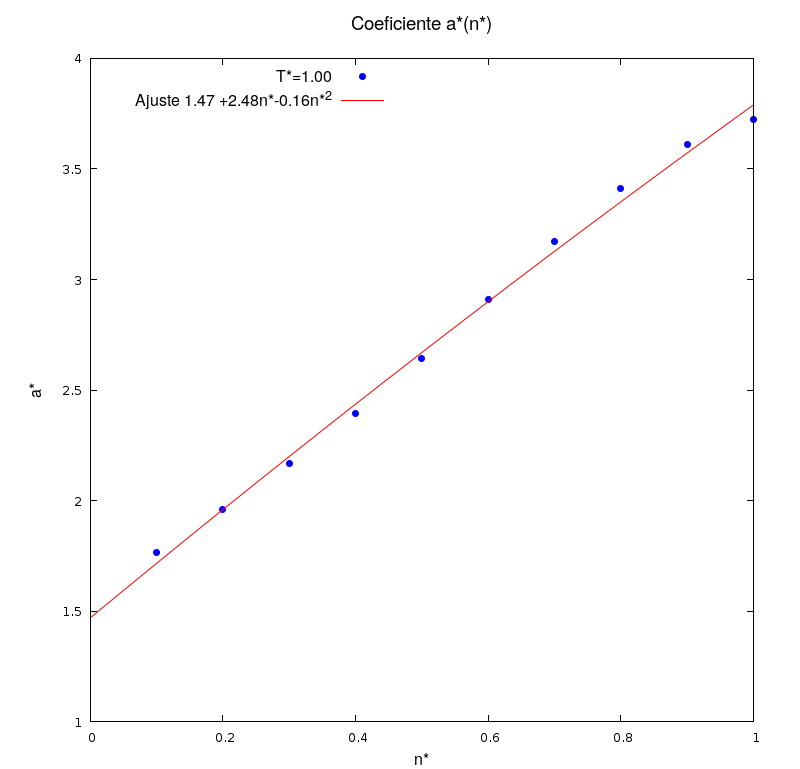
\includegraphics[width=0.49\linewidth]{ajusteT1.png}
	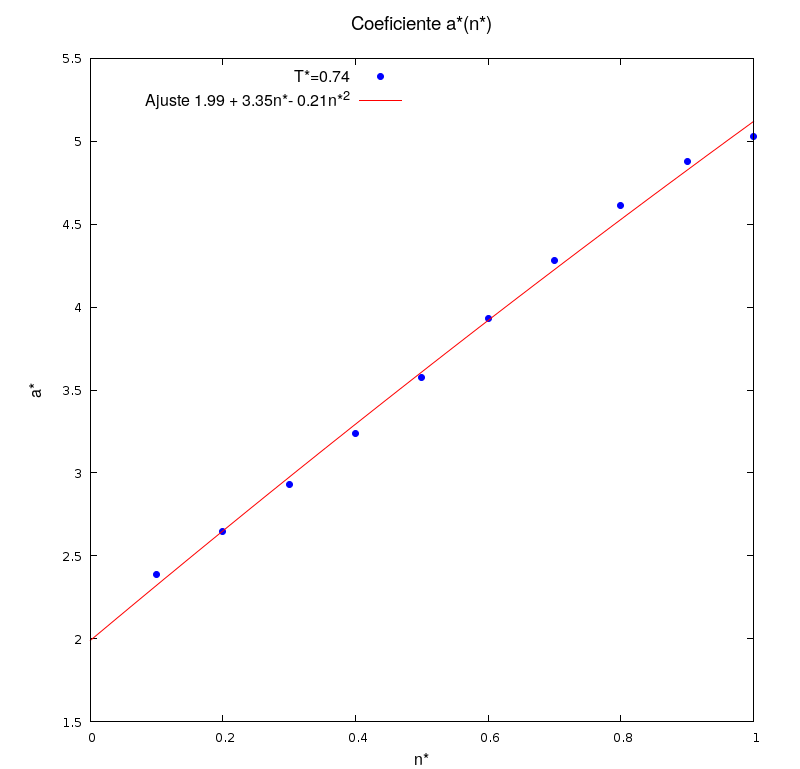
\includegraphics[width=0.49\linewidth]{ajusteT74.png}	
	\caption{Ajuste del Coeficiente $a^*$}
\end{figure}

\item[VIII.] \textbf{Ecuación de Presión con Teoría de Perturbaciones de Zwanzig}
Como ya conocemos la forma de las $a^*$, podemos calcular la ecuación de la presión a partir de la ecuación \eqref{Press_Red}.
\begin{equation*}
	p^* = n^* \left[ 1 + n^*b^*\right] - \left[ a^* + n^* \left(\frac{\partial a^*}{\partial n^*}\right)_{T^*} \right] {n^*}^2 
\end{equation*}


Se procedió a calcular la presión usando los dos casos de $T^*$. Lo que se obtuvo fue lo siguiente:
\begin{figure}[H]
	\centering
	\includegraphics[width=0.75\linewidth]{Isotermas.png}
	\caption{Isotermas de la presión de Zwanzig}
\end{figure}
Como escenario comparativo, se incluyeron las ecuaciones de Van Der Waals, Gas Ideal, Esferas Duras, junto a la de Teoría de Perturbaciones de Zwanzig. Se realizó para el caso de $T^*=0.74$
\begin{table}[H]
\centering
\begin{tabular}{|l|c|}
\hline 
Modelo & Ecuación de Presión \\ \hline 
Gas Ideal & $n^*$ \\ \hline 
Esfera Dura (HS) & $n^* \left[  1+\frac{2\pi}{3} n^* g_{hs}(1^+) \right] $\\ \hline 
Van Der Waals &  $\frac{n^*}{1-n^*b^*} - {n^*}^2a^*$ \\ \hline 
Zwanzig & $ p^*_{hs} - \left[ a^* + n^* \left(\frac{\partial a^*}{\partial n^*}\right)_{T^*} \right] {n^*}^2 $ \\ \hline 
\end{tabular} 
\caption{Ecuación de presión de diferentes modelos}
\end{table}
\begin{figure}[H]
	\centering 
	\includegraphics[width = 0.75\linewidth]{Comparar.png}
	\caption{Ecuaciones de Estados para el caso de $T^*=0.74$}
	\label{Fig:EcEst_Compara}
\end{figure}

\item[IX.]\textbf{Energía potencial promedio}

De la física estadística, con la teoría de Zwanzig para la función de partición es posible obtener una expresión para la energía media.
\begin{equation}
	Z_N \approx \left( V-Nb\right)^N e^{-\beta N a^*n^*}
\end{equation}
Siendo la energía promedio por partícula:
\begin{align}
	\overline{u} &= \frac{1}{N} \pd{\ln Z_n}{\beta}{} \nonumber\\
	&= \frac{1}{Z_N N} \pd{Z_n}{\beta}{} \nonumber \\
	&= \frac{ \left( V-Nb\right)^N e^{-\beta N a^*n^*} \left(-Nn^*a^*\right)  }{\left( V-Nb\right)^N e^{-\beta N a^*n^*} N}  \nonumber \\
	\overline{u} &= -a^*n^*
\end{align}
	






\end{enumerate}

\pagebreak




\bibliographystyle{plain}
\bibliography{biblio}


\end{document}

